\textit{This section was contributed by John Naliboff, Cedric Thieulot and Marcel Saaro}

This benchmark originates in the book of Gerya \cite{gery10}. 
In the first edition of the book the domain is a square of size 
$L=1000~\si{\km}$, while it is of size $L=100~\si{\km}$ in the second, which is the dimension we use in this benchmark. The boundary conditions and material layout are shown in Figure~\ref{fig:shortening_vp_block}.

\begin{figure}[htp!]
\centering
\input{tikz/shortening_block}
\caption{\it Shortening of visco-(elasto-)plastic block benchmark. Boundary conditions and material layout. }
\label{fig:shortening_vp_block}
\end{figure}

The thickness of the top and bottom weak layer
as well as the dimensions of the square inclusion have been modified so 
that element edges align with these material interfaces 
for uniformly refined meshes of level 4 and up: The size of the inclusion is then $L/8=12.5~\si{\km}$ and the block has a thickness of $50~\si{km}$.

The velocity on the boundaries is $v_{bc}=5\cdot 10^{-9}~\si{\meter\per\second}$ so that the background strain rate is  
$2 v_{bc}/L = 10^{-13}~\si{\per\second}$.
The weak medium and the weak inclusion have a viscosity 
$\eta=10^{17}~\si{\pascal\second}$ while 
the block is visco-plastic with $c=100~\si{\mega\pascal}$ and $\phi=37\si{\degree}$. 
Gravity is set to zero (material density values are then irrelevant) and pressure is required to have a zero volume average.

In the case of the von Mises ($\phi=0\si{\degree}$) failure criterion we expect the shear bands at $\frac{\pi}{4}=45\si{\degree}$ (see green line in Figure~\ref{fig:shortening_vp_block}). 
When $\phi=37\si{\degree}$, we expect the shear band angle to be 
given by the Coulomb angle $\frac{\pi}{4} +\pm \frac{\phi}{2}$, i.e. 26.5\si{\degree} in compression and 63.5\si{\degree} in extension
represented by the blue lines in Figure~\ref{fig:shortening_vp_block}. 


There are 3 input files in \verb|/benchmarks/viscoelastic_plastic_shear_bands/gerya_2019|.

The \verb|gerya_2019_vp.prm| file corresponds to the visco-plastic case, while \verb|gerya_2019_vep.prm| corresponds to the visco-elasto-plastic case and \verb|gerya_2019_vp_damper.prm| 
corresponds to the visco-plastic case which makes use of the so-called plastic damper.

% {\color{red}say something about authorising negative pressure parameter ?}

In order to easy compare between models, the strain rate is measured on the purple dashed line and plotted with the help of the included script: \verb|gerya_2019_analysis.py|.


\begin{figure}[h]
\centering
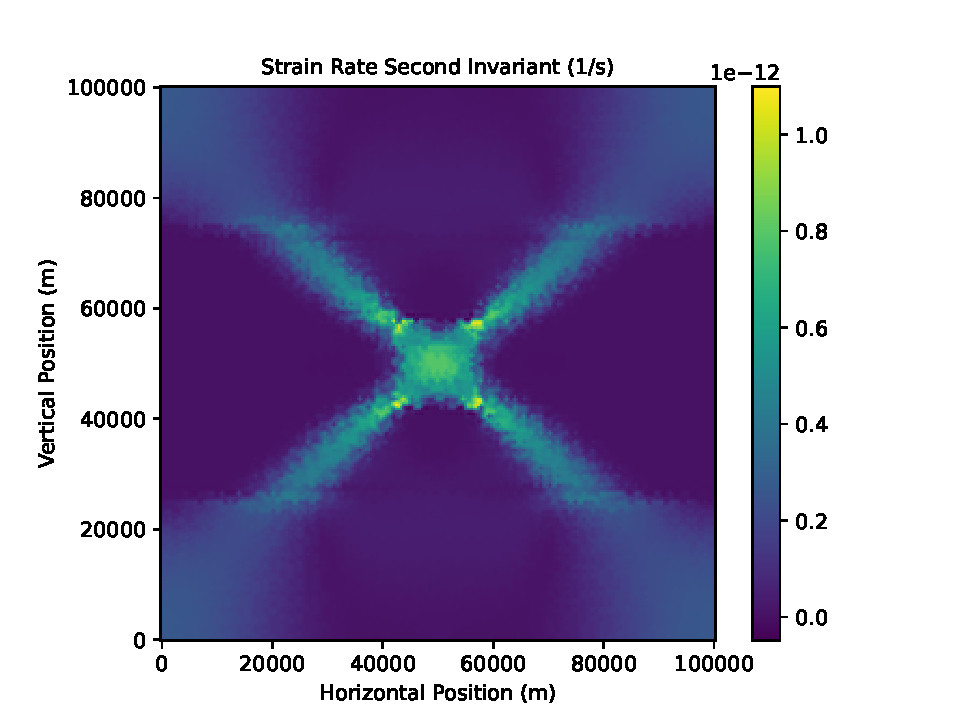
\includegraphics[width=6cm]{gerya_2019_damper/strain_rate_field.pdf}
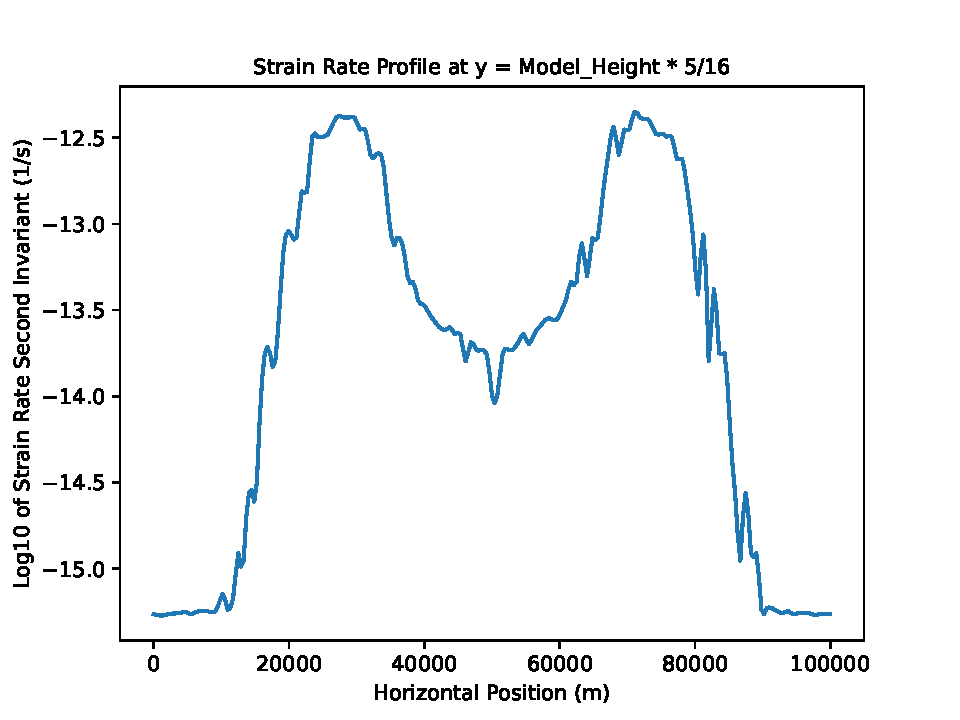
\includegraphics[width=6cm]{gerya_2019_damper/strain_rate_profile.pdf}
\caption{}
\label{fig:gerya_2019_damper_results}
\end{figure}

\begin{figure}[h]
\centering
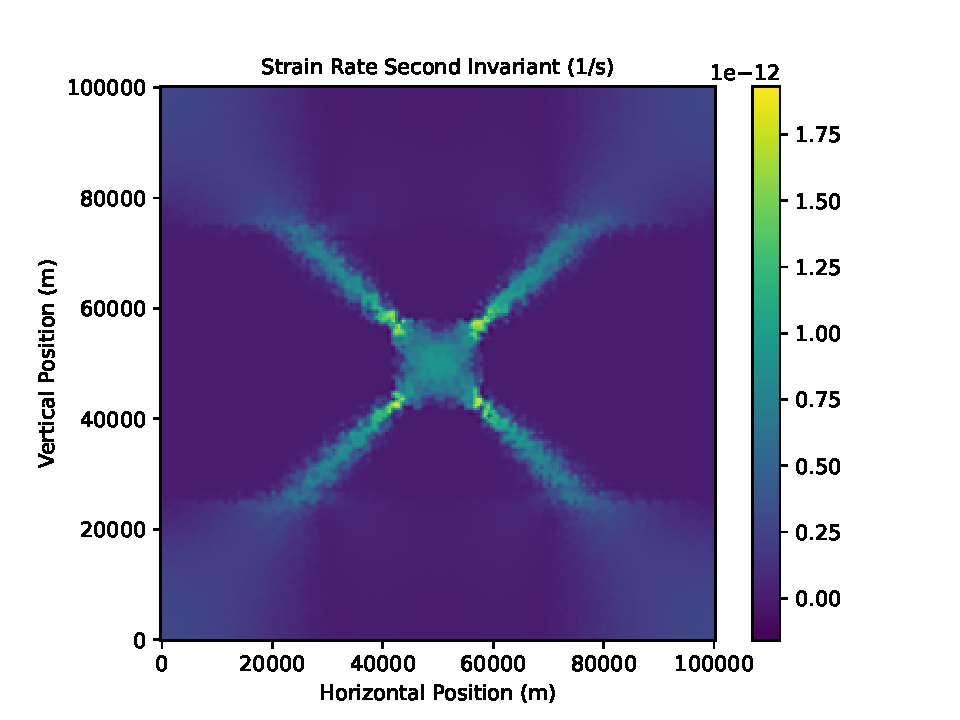
\includegraphics[width=6cm]{gerya_2019_vp/strain_rate_field.pdf}
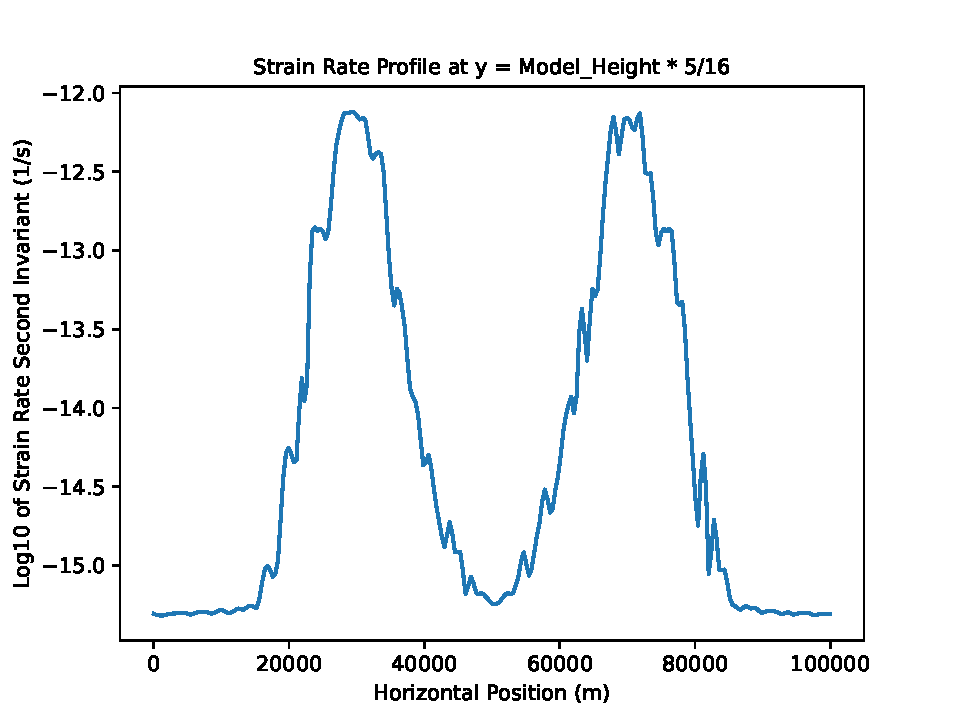
\includegraphics[width=6cm]{gerya_2019_vp/strain_rate_profile.pdf}
\caption{}
\label{fig:gerya_2019_vp_results}
\end{figure}

\begin{figure}[h]
\centering
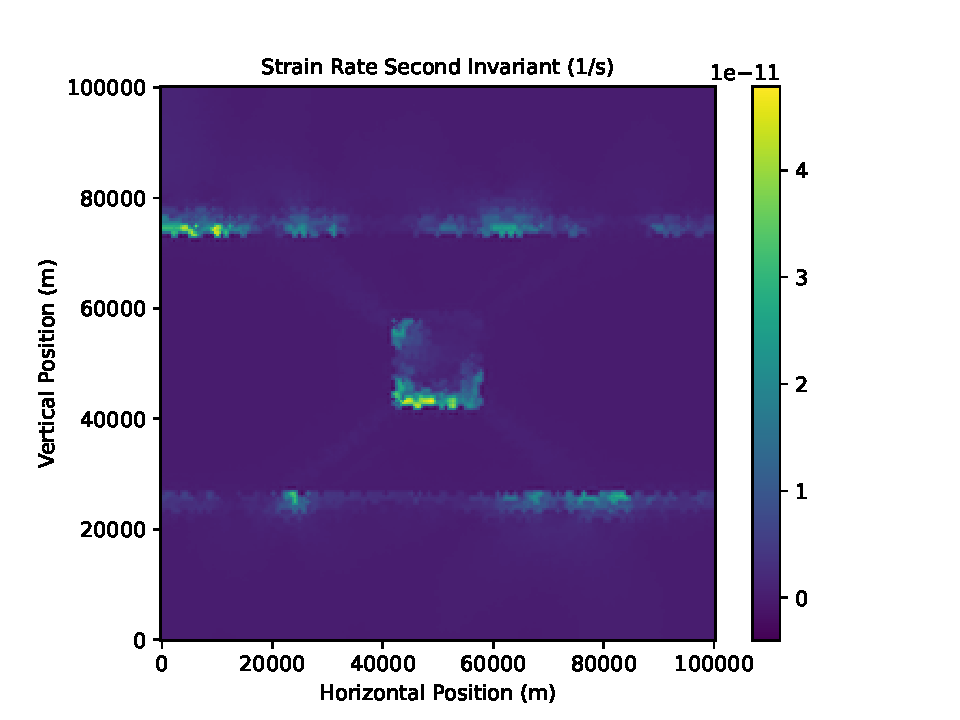
\includegraphics[width=6cm]{gerya_2019_vep/strain_rate_field.pdf}
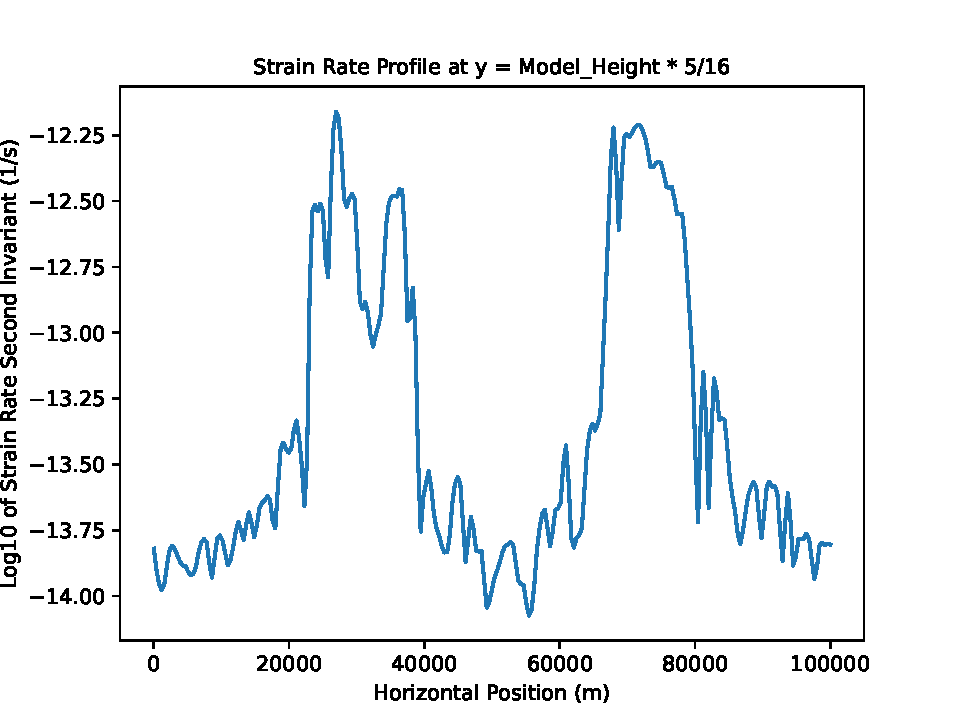
\includegraphics[width=6cm]{gerya_2019_vep/strain_rate_profile.pdf}
\caption{}
\label{fig:gerya_2019_vep_results}
\end{figure}